\documentclass[times, utf8, seminar]{fer}
\usepackage{booktabs}
%math packages
\usepackage{authblk}
\usepackage{mathtools}
\usepackage{amsmath}
\usepackage[binary-units=true]{siunitx}
%table of images
\usepackage{graphicx}
\usepackage{longtable}
\usepackage{adjustbox}

%%floor symbol
\DeclarePairedDelimiter\floor{\lfloor}{\rfloor}

%%SI unit notation
\makeatletter
\providecommand\add@text{}
\newcommand\tagaddtext[1]{%
  \gdef\add@text{#1\gdef\add@text{}}}% 
\renewcommand\tagform@[1]{%
  \maketag@@@{\llap{\add@text\quad}(\ignorespaces#1\unskip\@@italiccorr)}%
}
\makeatother


\begin{document}

% TODO: Navedite naslov rada.
\title{Uporaba steganografije u revezibilnoj deidentifikaciji}

% TODO: Navedite vaše ime i prezime.
\author{	Katarina Matić,
	Hrvoje Backović,
	Marin Oršić,\\
	Dino Rakipović,
	Ivan Relić,
	Filip Reškov	}

% TODO: Navedite ime i prezime mentora.

\voditelj{Slobodan Ribarić}

\maketitle

\tableofcontents

\chapter{Projektni zadatak}
\section{Opis projektnog zadatka}
\section{Pregled i opis srodnih rješenja}
\section{Konceptualno rješenje zadatka}

\chapter{Postupak rješavanja zadataka}

\chapter{Ispitivanje rješenja}
Razvijeni sustav za steganografski postupak, kao i svi steganografski algoritmi, ograničen je količinom podataka koja se može upisati u neku sliku. Ova granica prvenstveno je određena veličinom slike, a određuju je i odabir kanala te najznačajniji bit do kojeg se upisuju podaci. Glavna ideja steganografskog algoritma jest upisati podatak u sliku bez velikog utjecaja na konačni izgled. Drugim riječima, izgled konačne slike uvjetovan je količinom podataka koji se u nju upisuju. Potrebno je pronaći dobre parametre steganografskog algoritma koji nude dobara kapacitet skrivenih podataka, a neznatno žrtvuju kvalitetu izvorne slike.
\par
Parametri algoritma koji su podešavani u ispitivanju su:
\begin{itemize}
\item Najznačajniji bit do kojeg se slijedno upisuje podatak
\item RGB komponente u koje će se upisivati podaci
\end{itemize}
Algoritam \textit{Least Significant Bit(LSB)} upisivanje sadržaja započinje s bitovima najnižeg značaja. Razlog tome leži u tome što se izmjenom bita najmanjeg značaja piksel najmanje mijenja. Praktični primjer bio bi kada bismo odlučili mijenjati samo B(\textit{blue}) komponentu i to samo najniži bit svakog bajta. Za svaki piksel slike(3 komponente, svaka po 1 bajt) dobije se jedan bit prostora za skrivanje podataka. Općenito, količina podataka koja se može upisati($n_{data}$), u ovisnosti o broju komponenti za upisivanje $n_{components}$ i broja najnižih bitova svake odabrane komponente za upisivanje $n_{bits}$ te veličini(broju piksela) $n_{pixels}$ slike je:
\begin{equation}
\label{num_bits}
n_{data} = \floor{\cfrac{n_{pixels} \cdot n_{components} \cdot n_{bits}}{8}}
\tagaddtext{[B]}
\end{equation}
\par
Udio veličine podataka $\eta$ koje je za dane parametre moguće upisati u sliku u odnosu na ukupnu veličinu slike je:
\begin{equation}
\label{eta}
\eta = \cfrac{n_{data}}{3 \cdot n_{pixels}} = \cfrac{n_{components} \cdot n_{bits}}{24}
\end{equation}
Povećanjem $\eta$ vizualna razlika između izvorne slike i slike obrađene steganografskim algoritmom, u našem slučaju \textit{LSB}-om, povećava se. U nastavku slijede rezultati ispitivanja odnosa izvorne i obrađene slike u ovisnosti o parametrima $n_{components}$ i $n_{bits}$.
\section{Ispitna baza}
Ispitivanje algoritma \textit{LSB} napravljeno je nad dvjema različitim slikama. Slika \ref{chart_original} korištena je kako bi se ispitala osjetljivost boja na postupak, dok bi slika \ref{pattern_original} trebala pokazati osjetljivost tekstura. Ispitni primjeri pripremljeni su u ovisnosti o parametrima $n_{components}$ i $n_{bits}$. Za obje izvorne slike algoritam je pokrenut za sve moguće kombinacije parametara. Parametar $n_{components}$ poprima vrijednosti iz $[1,3]$, pošto svaki piksel ima crvenu, zelenu i plavu komponentu boje. Parametar $n_{bits}$ poprima vrijednosti iz $[1,8]$, gdje se za svaki bajt koristi $n_{bits}$ bitova u koje se upisuje podatak. Ukupno postoje 24 moguća para parametara algoritma. Nadalje, za svaki ispitni primjer odabrana je najveća količina podataka moguća za dane parametre, te su generirani nizovi bitova nasumične vrijednosti. U idućem odjeljku slijede rezultati ispitivanja, koji vizualno prikazuju promjenu kvalitete slike u ovisnosti o parametrima algoritma.
\begin{center}
\begin{figure}[ht]
	\caption{Izvorna slika jednostavnih boja, bez teksture}
	\label{chart_original}
	\centerline{
	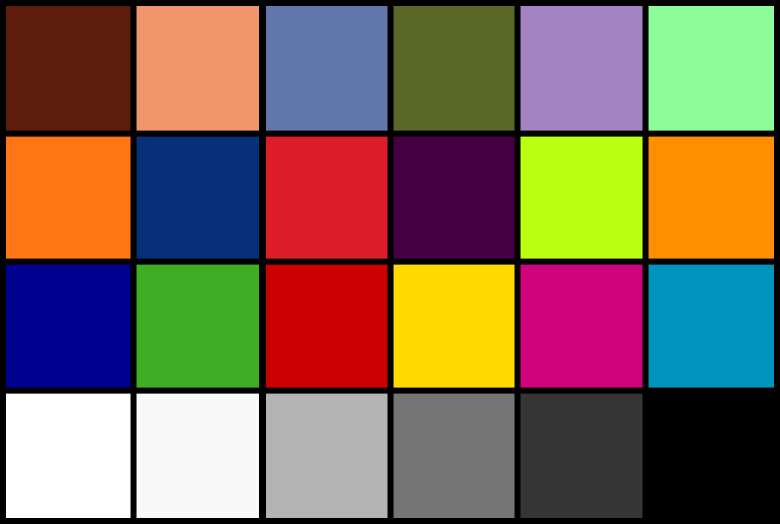
\includegraphics[scale=0.4]{../benchmark_results/color_chart/original.png}	
	}
\end{figure}
\end{center}

\begin{center}

\begin{figure}[ht]
	\caption{Izvorna slika s teksturom}
	\label{pattern_original}
	\centerline{
	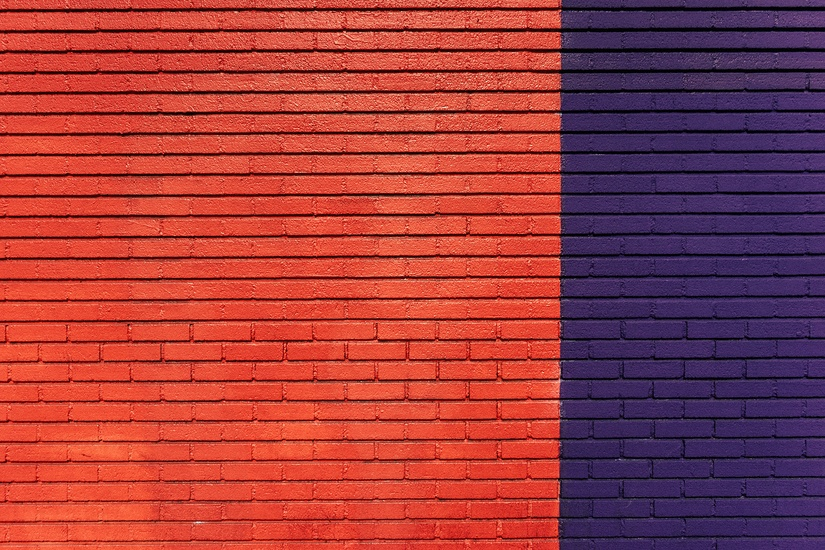
\includegraphics[scale=0.4]{../benchmark_results/pattern/pattern_original.jpg}	
	}
\end{figure}
\end{center}

\section{Rezultati ispitivanja}
Tablice \ref{pattern_original} i \ref{table_chart} prikazuju obređene slike algoritmom \textit{LSB} za vrijednosti parametara $n_{components}$ i $n_{bits}$. Treći stupac, $\eta$, prikazuje udio upisanih podataka u ukupnoj veličini slike.
\begin{center}
\begin{longtable}{|c|c|c|c|}
\caption{Osjetljivost kvalitete slike jednostavnih boja na \textit{LSB} u ovisnosti o parametrima $n_{components}$ i $n_{bits}$}\\
\hline
\textbf{$n_{components}$} & \textbf{$n_{bits}$} & \textbf{$\eta$} & \textbf{Slika}\\
\hline
\label{table_chart}
\endfirsthead
\multicolumn{4}{c}%
{\tablename\ \thetable\ -- \textit{Nastavljeno s prethodne strane}} \\
\hline
\textbf{$n_{components}$} & \textbf{$n_{bits}$} & \textbf{$\eta$} & \textbf{Slika}\\
\hline
\endhead
\hline \multicolumn{4}{r}{\textit{Nastavlja se na idućoj strani}} \\
\endfoot
\hline
\endlastfoot
1 & 1 &4\% & 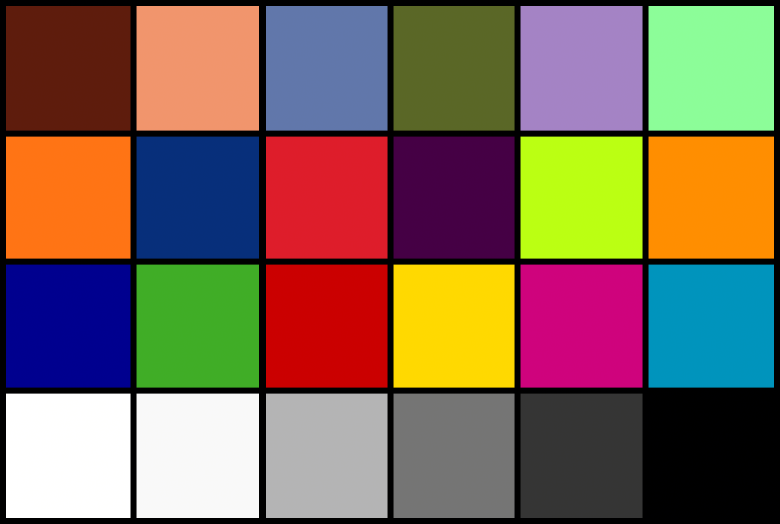
\includegraphics[scale=0.3]{../benchmark_results/color_chart/1_components-1_bits.png} \\
1 & 2 &8\% & 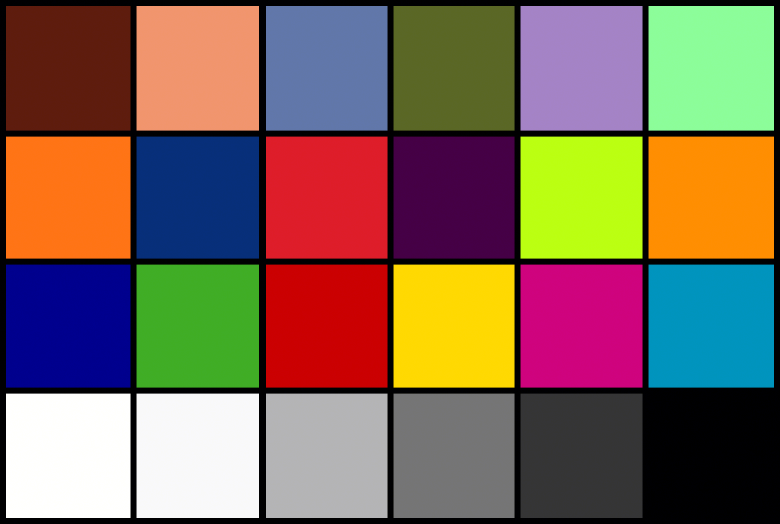
\includegraphics[scale=0.3]{../benchmark_results/color_chart/1_components-2_bits.png} \\
1 & 3 &12\% & 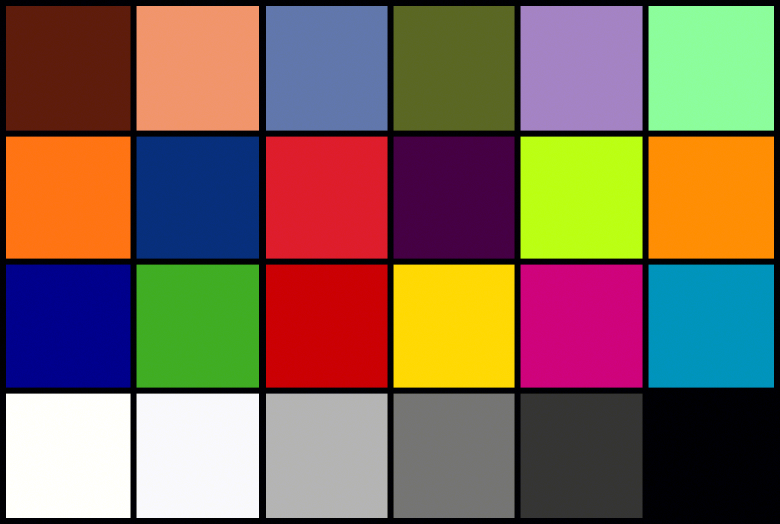
\includegraphics[scale=0.3]{../benchmark_results/color_chart/1_components-3_bits.png} \\
1 & 4 &17\% & 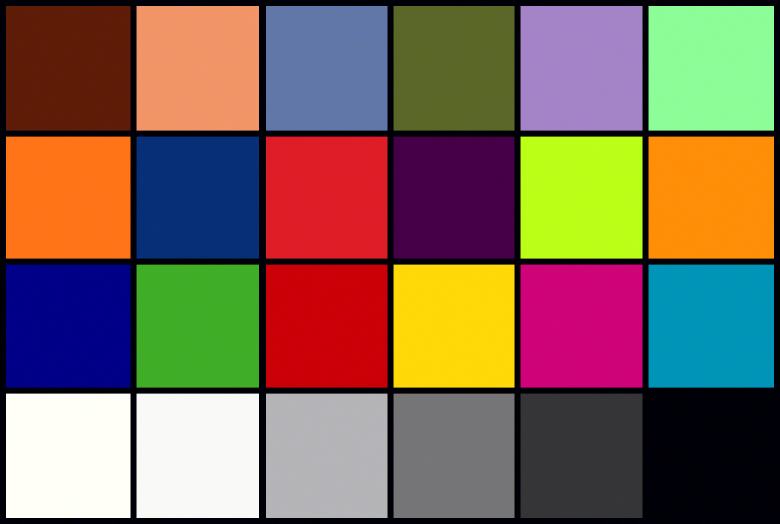
\includegraphics[scale=0.3]{../benchmark_results/color_chart/1_components-4_bits.png} \\
1 & 5 &21\% & 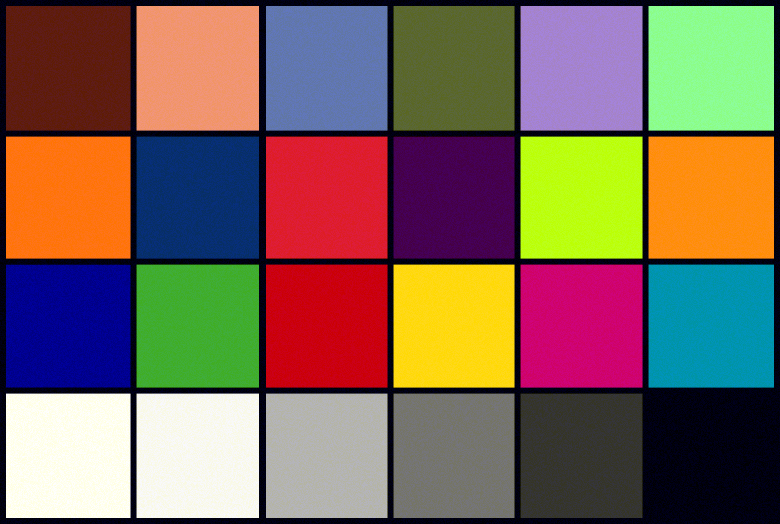
\includegraphics[scale=0.3]{../benchmark_results/color_chart/1_components-5_bits.png} \\
1 & 6 &25\% & 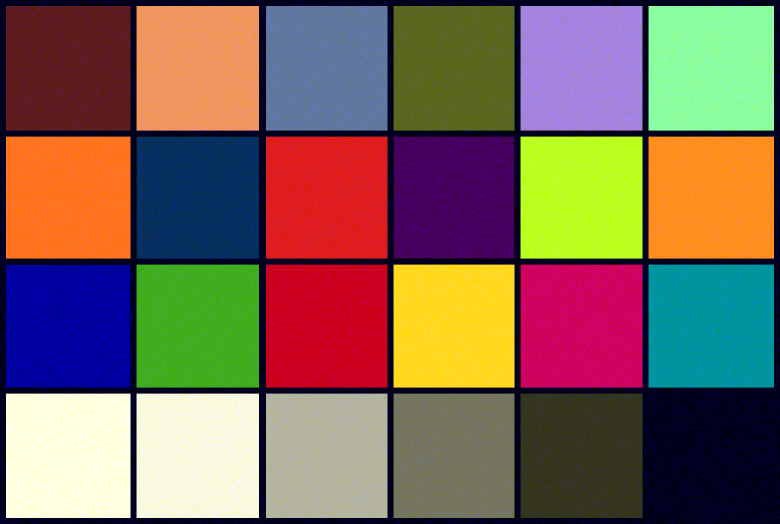
\includegraphics[scale=0.3]{../benchmark_results/color_chart/1_components-6_bits.png} \\
1 & 7 &29\% & 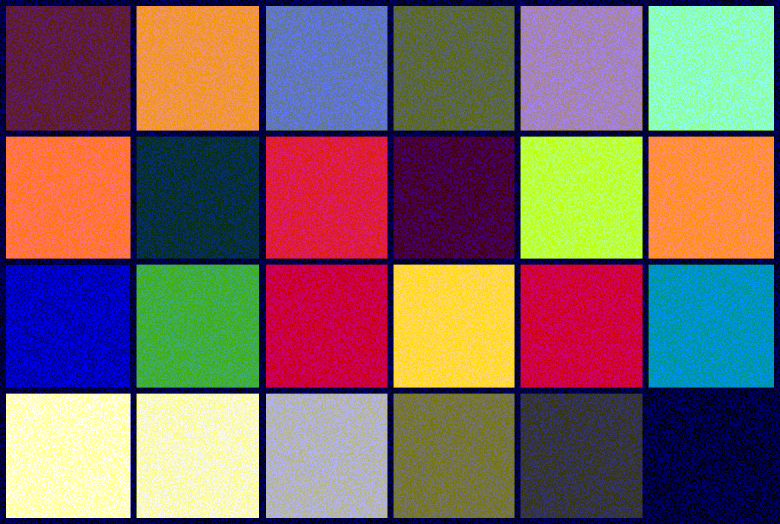
\includegraphics[scale=0.3]{../benchmark_results/color_chart/1_components-7_bits.png} \\
1 & 8 &33\% & 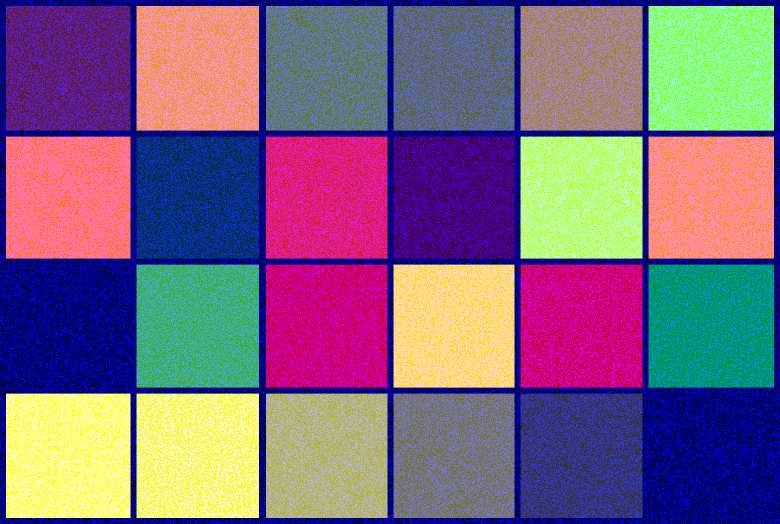
\includegraphics[scale=0.3]{../benchmark_results/color_chart/1_components-8_bits.png} \\
2 & 1 &8\% & 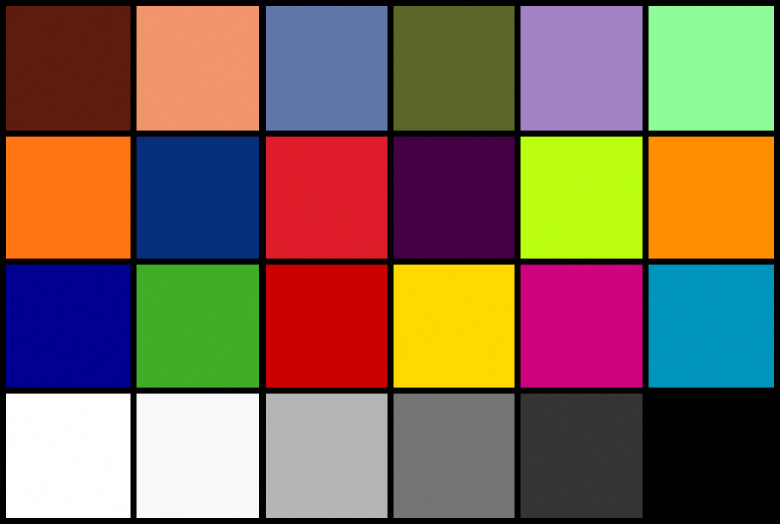
\includegraphics[scale=0.3]{../benchmark_results/color_chart/2_components-1_bits.png} \\
2 & 2 &12\% & 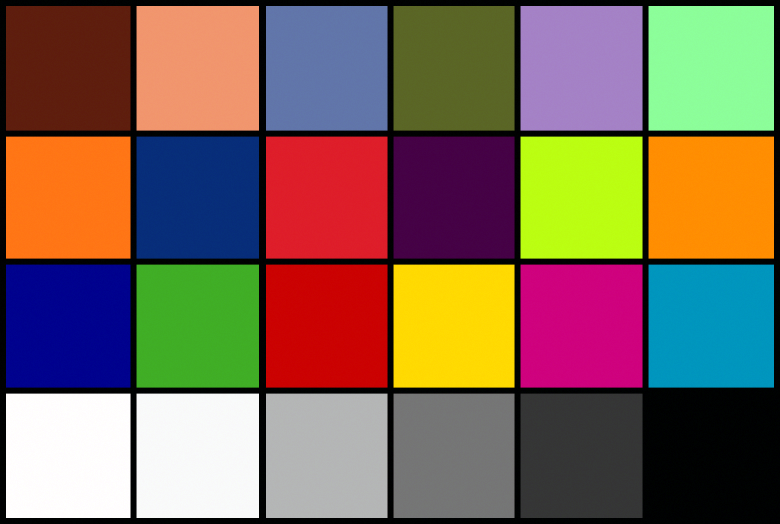
\includegraphics[scale=0.3]{../benchmark_results/color_chart/2_components-2_bits.png} \\
2 & 3 &25\% & 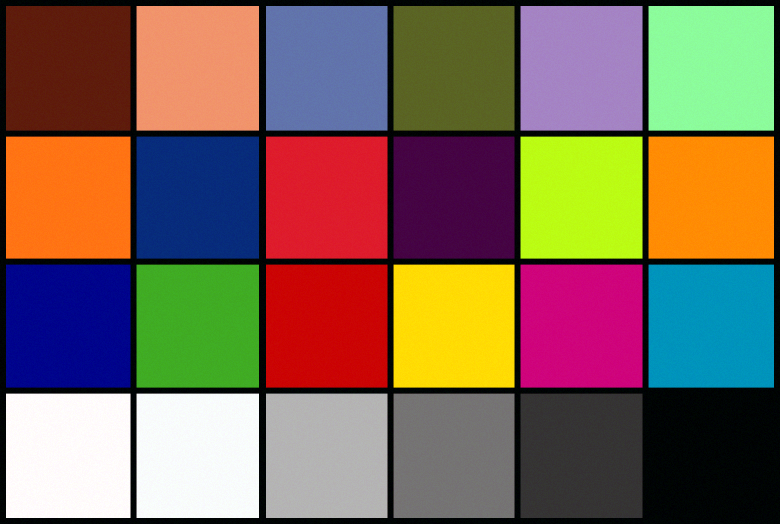
\includegraphics[scale=0.3]{../benchmark_results/color_chart/2_components-3_bits.png} \\
2 & 4 &33\% & 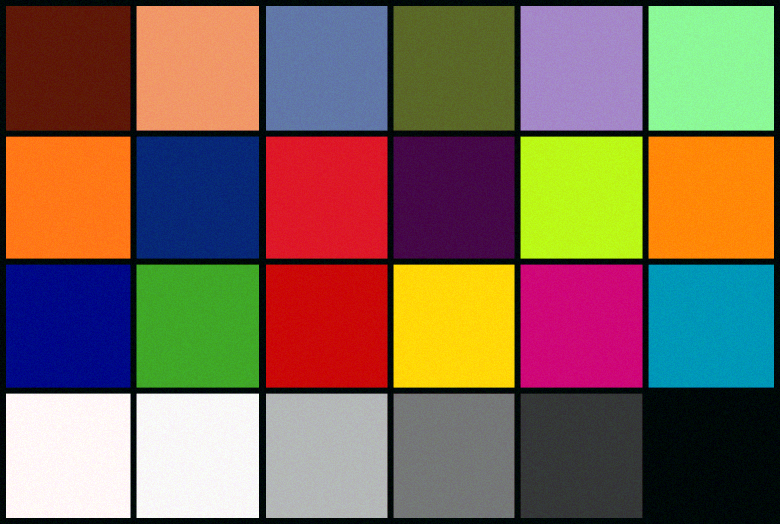
\includegraphics[scale=0.3]{../benchmark_results/color_chart/2_components-4_bits.png} \\
2 & 5 &42\% & 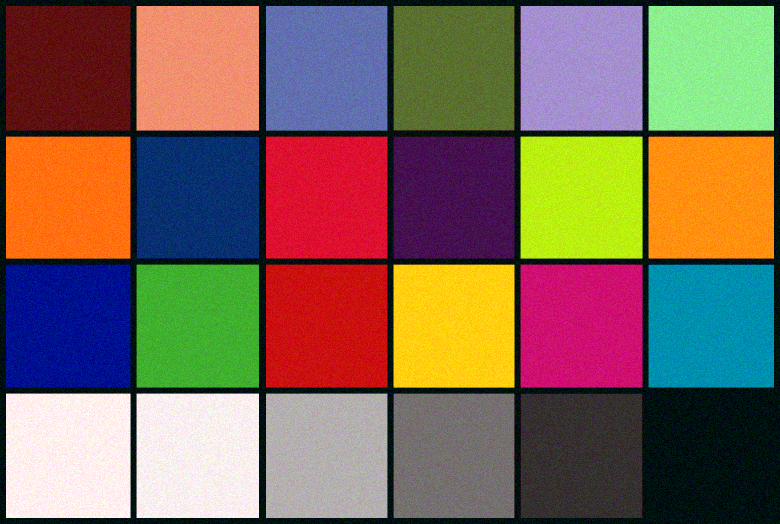
\includegraphics[scale=0.3]{../benchmark_results/color_chart/2_components-5_bits.png} \\
2 & 6 &50\% & 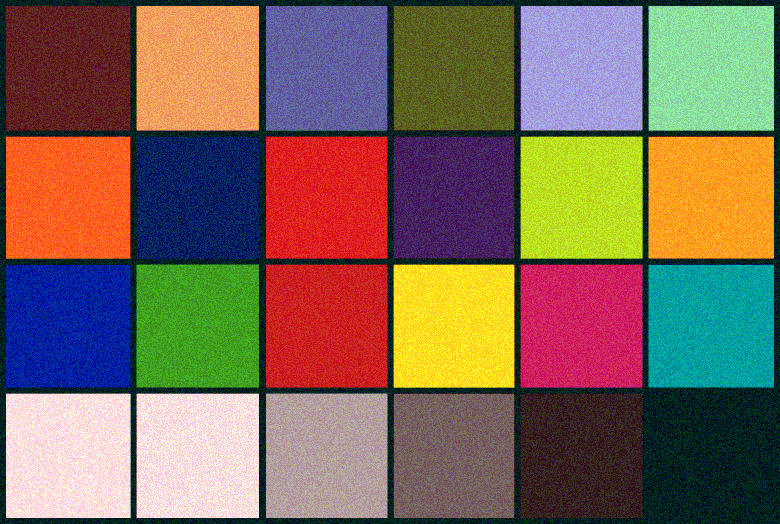
\includegraphics[scale=0.3]{../benchmark_results/color_chart/2_components-6_bits.png} \\
2 & 7 &58\% & 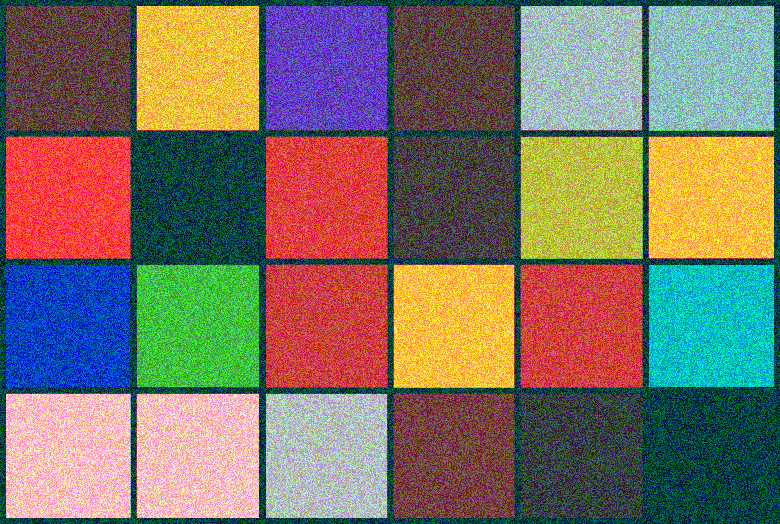
\includegraphics[scale=0.3]{../benchmark_results/color_chart/2_components-7_bits.png} \\
2 & 8 &67\% & 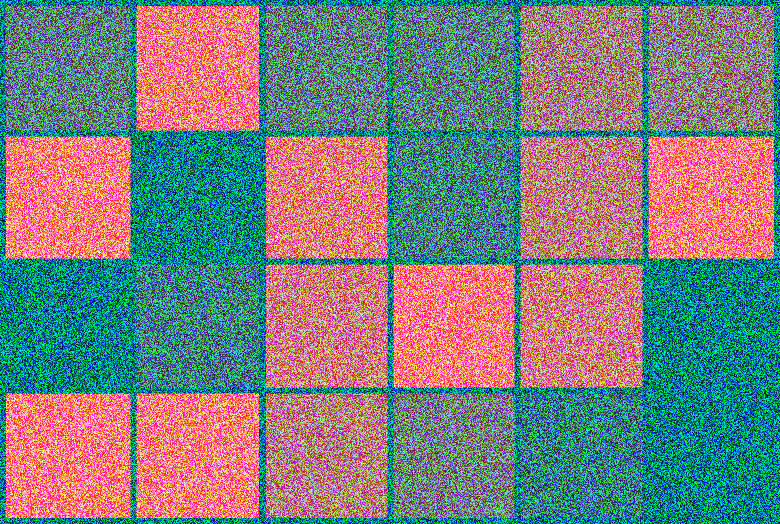
\includegraphics[scale=0.3]{../benchmark_results/color_chart/2_components-8_bits.png} \\
3 & 1 &12\% & 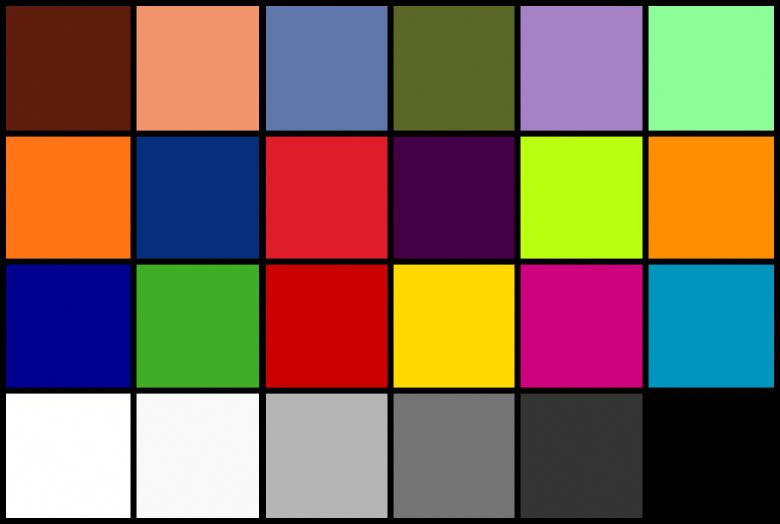
\includegraphics[scale=0.3]{../benchmark_results/color_chart/3_components-1_bits.png} \\
3 & 2 &25\% & 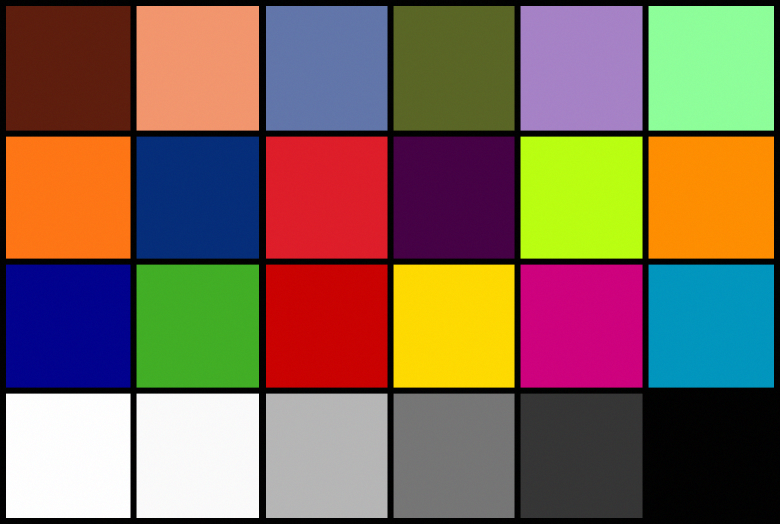
\includegraphics[scale=0.3]{../benchmark_results/color_chart/3_components-2_bits.png} \\
3 & 3 &38\% & 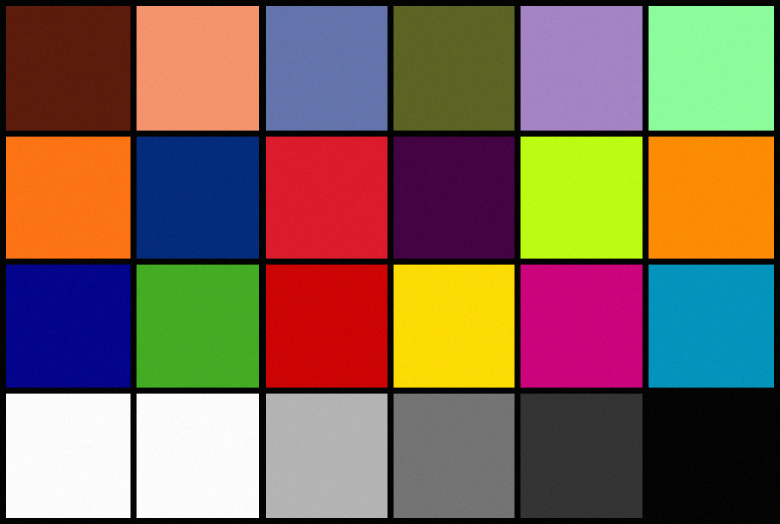
\includegraphics[scale=0.3]{../benchmark_results/color_chart/3_components-3_bits.png} \\
3 & 4 &50\% & 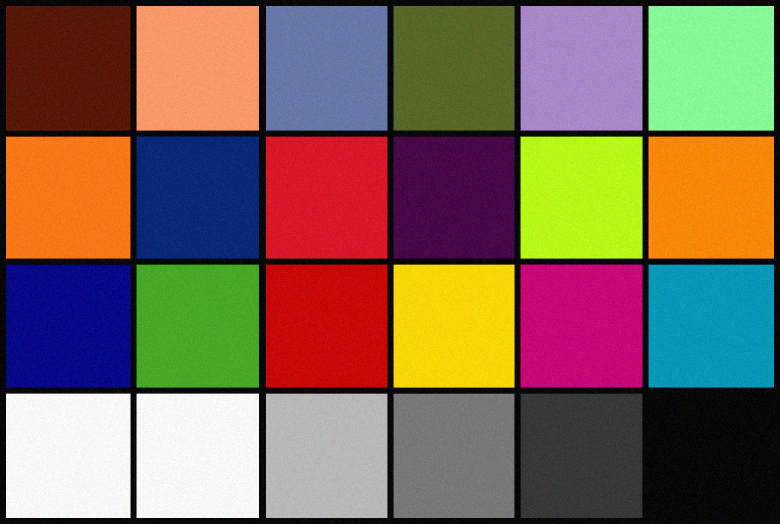
\includegraphics[scale=0.3]{../benchmark_results/color_chart/3_components-4_bits.png} \\
3 & 5 &62\% & 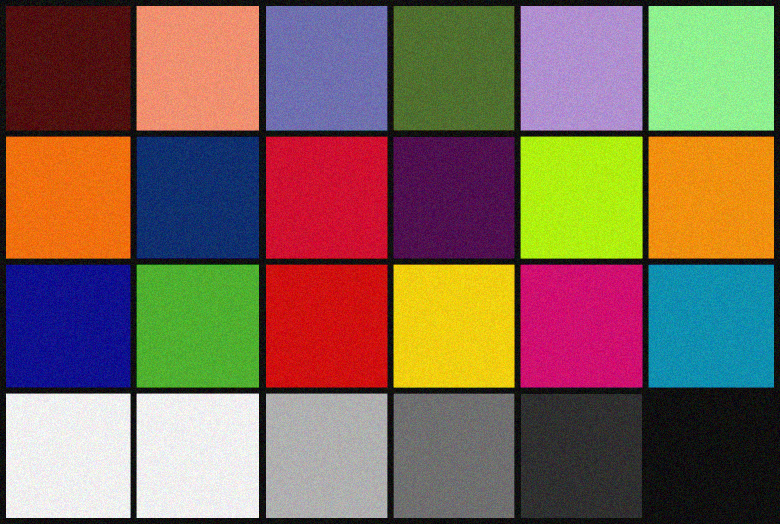
\includegraphics[scale=0.3]{../benchmark_results/color_chart/3_components-5_bits.png} \\
3 & 6 &75\% & 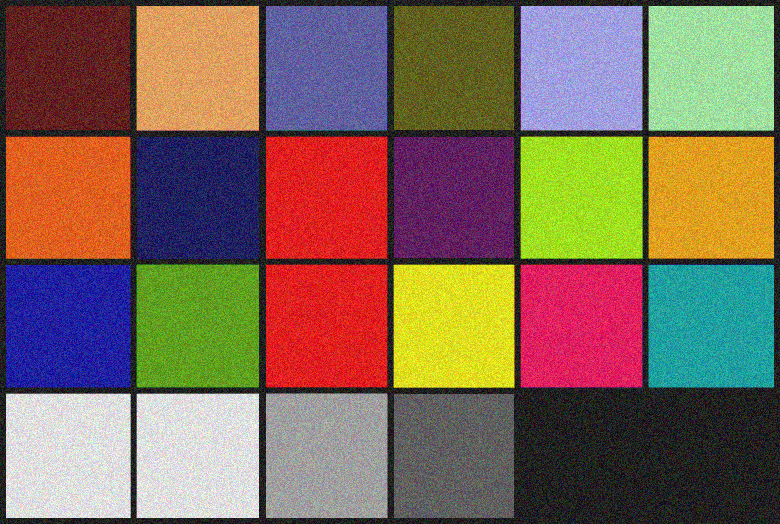
\includegraphics[scale=0.3]{../benchmark_results/color_chart/3_components-6_bits.png} \\
3 & 7 &88\% & 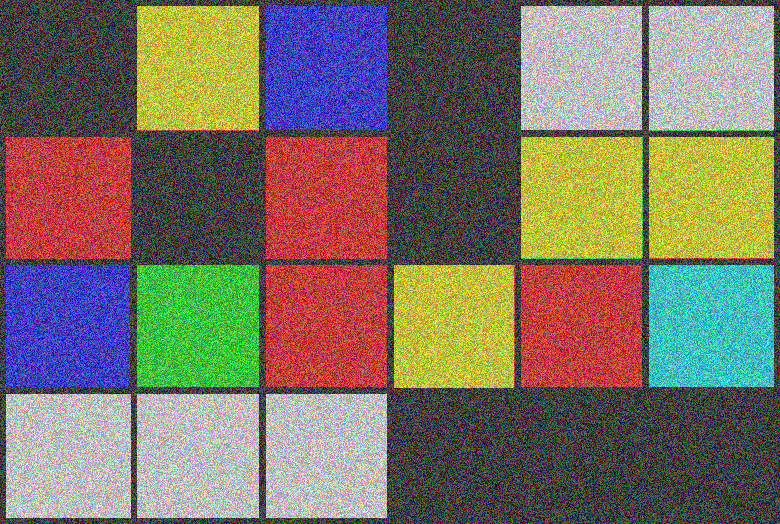
\includegraphics[scale=0.3]{../benchmark_results/color_chart/3_components-7_bits.png} \\
3 & 8 &100\% & 
\includegraphics[scale=0.3]{../benchmark_results/color_chart/3_components-8_bits.png} \\
\end{longtable}
\end{center}

\begin{center}
\begin{longtable}{|c|c|c|c|}
\caption{Osjetljivost kvalitete slike tekstura na \textit{LSB} u ovisnosti o parametrima $n_{components}$ i $n_{bits}$}\\
\hline
\textbf{$n_{components}$} & \textbf{$n_{bits}$} & \textbf{$\eta$} & \textbf{Slika}\\
\hline
\label{table_pattern}
\endfirsthead
\multicolumn{4}{c}%
{\tablename\ \thetable\ -- \textit{Nastavljeno s prethodne strane}} \\
\hline
\textbf{$n_{components}$} & \textbf{$n_{bits}$} & \textbf{$\eta$} & \textbf{Slika}\\
\hline
\endhead
\hline \multicolumn{4}{r}{\textit{Nastavlja se na idućoj strani}} \\
\endfoot
\hline
\endlastfoot
1 & 1 &4\% & 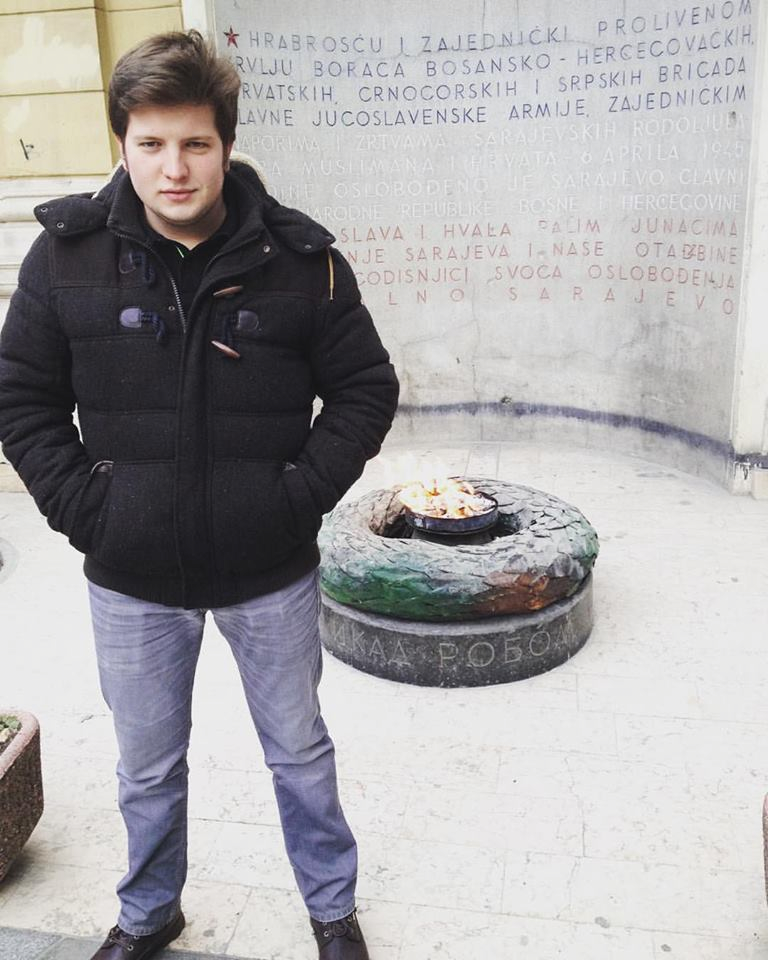
\includegraphics[scale=0.3]{../benchmark_results/pattern/1_components-1_bits.png} \\
1 & 2 &8\% & 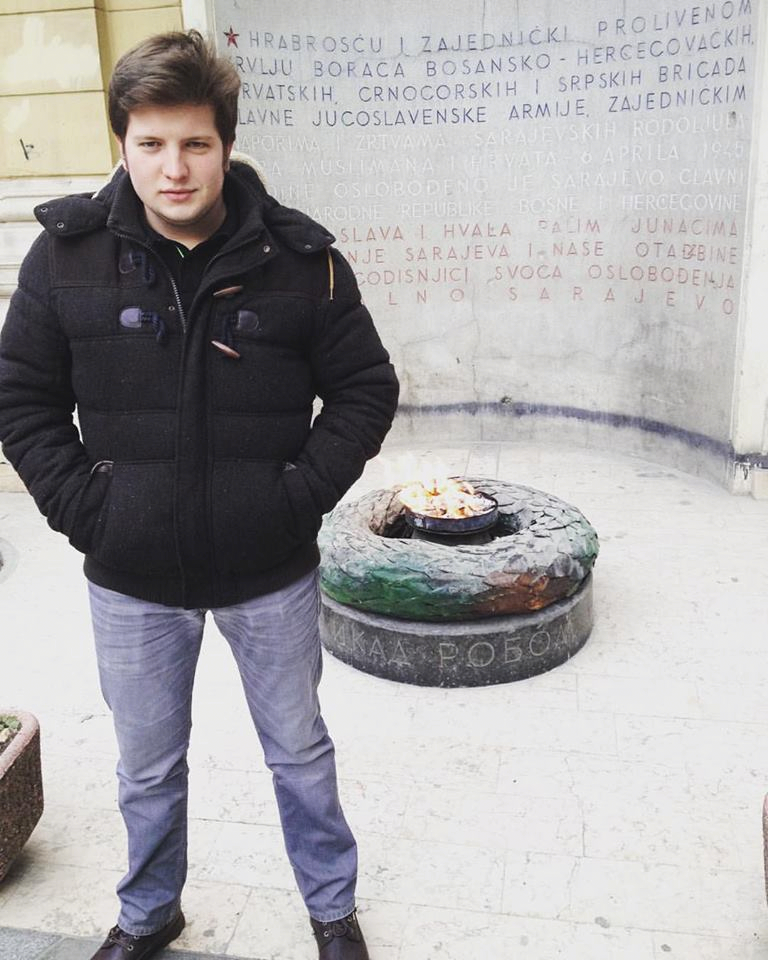
\includegraphics[scale=0.3]{../benchmark_results/pattern/1_components-2_bits.png} \\
1 & 3 &12\% & 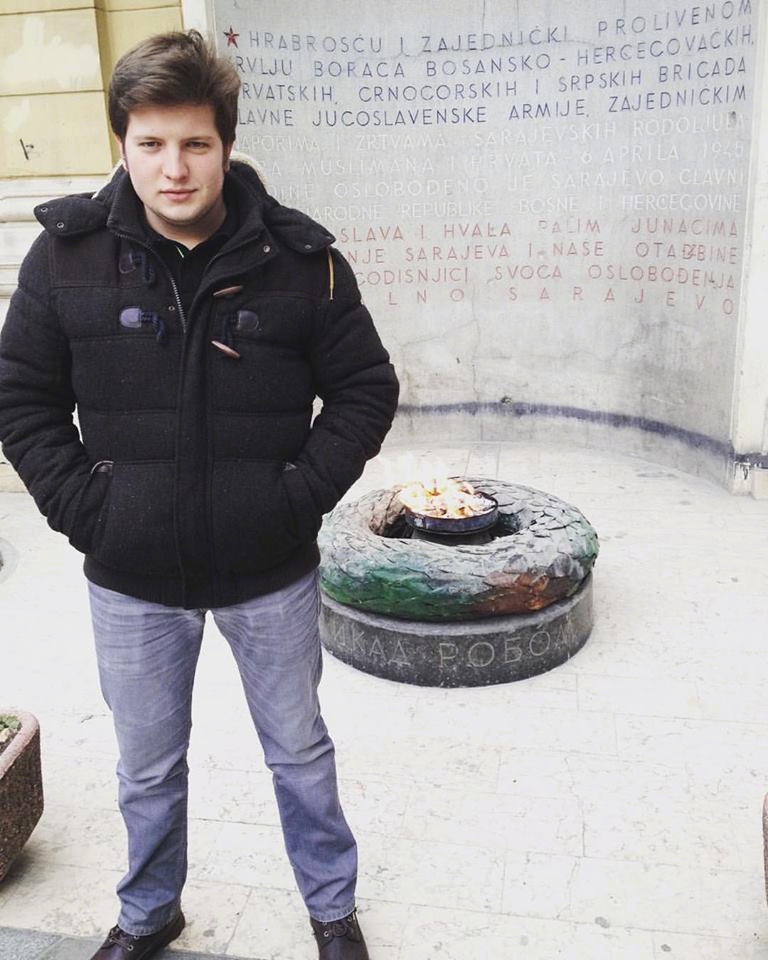
\includegraphics[scale=0.3]{../benchmark_results/pattern/1_components-3_bits.png} \\
1 & 4 &17\% & 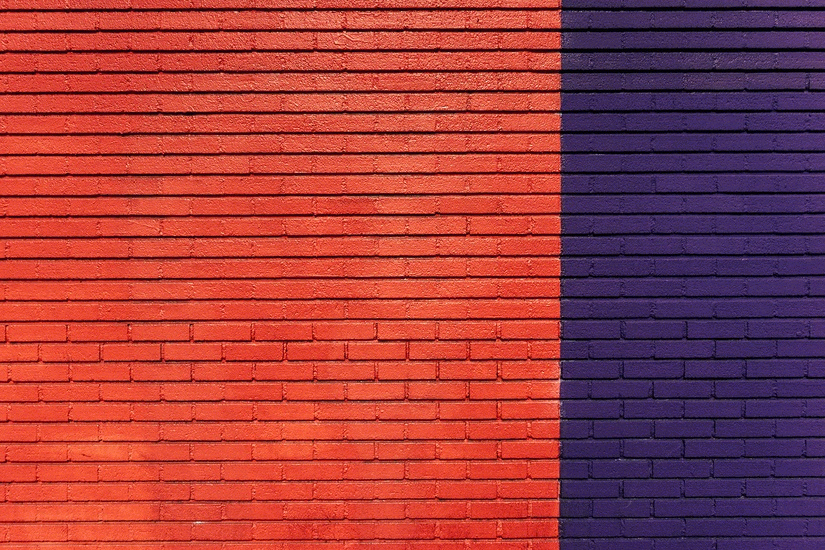
\includegraphics[scale=0.3]{../benchmark_results/pattern/1_components-4_bits.png} \\
1 & 5 &21\% & 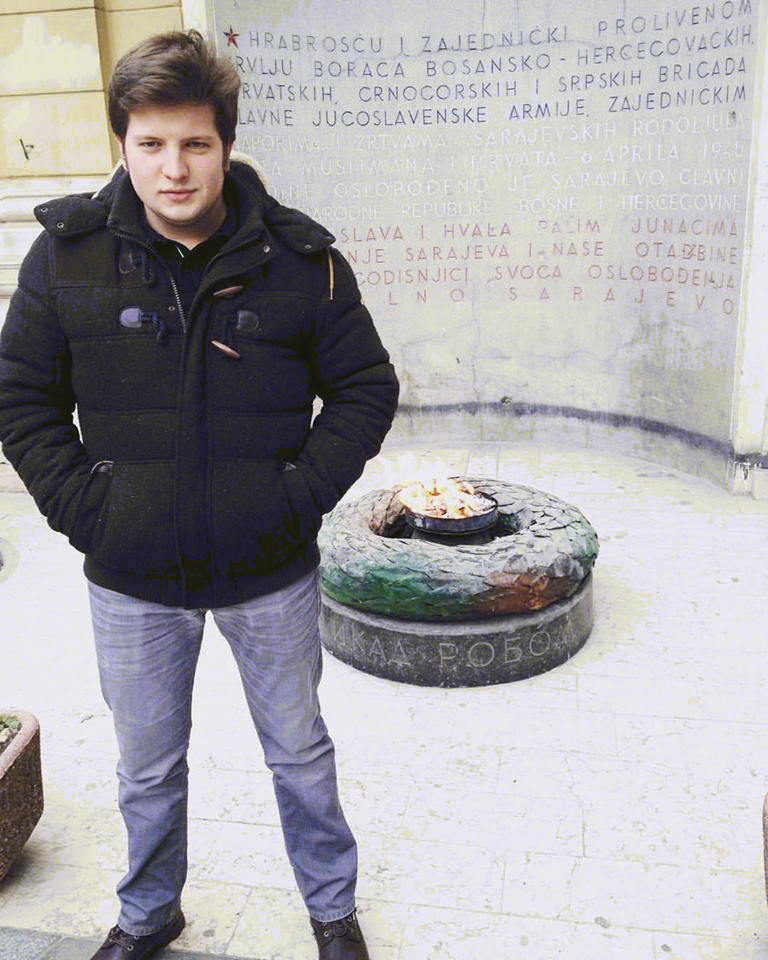
\includegraphics[scale=0.3]{../benchmark_results/pattern/1_components-5_bits.png} \\
1 & 6 &25\% & 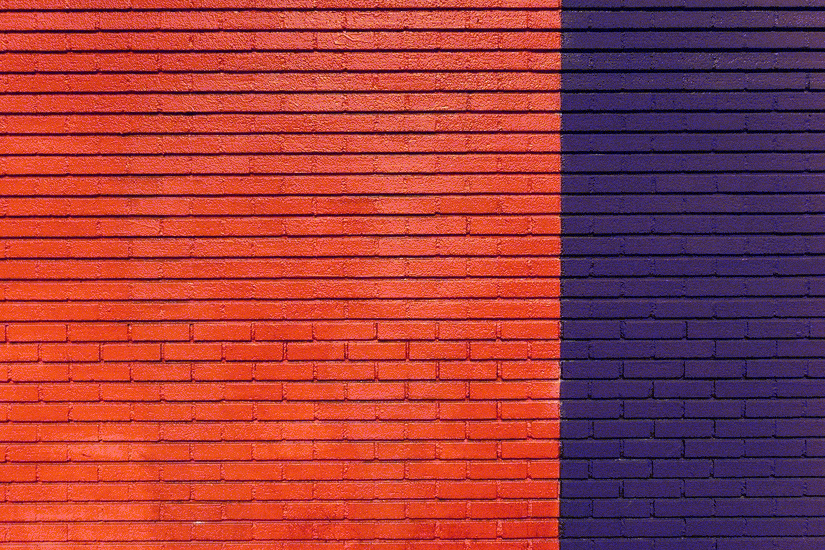
\includegraphics[scale=0.3]{../benchmark_results/pattern/1_components-6_bits.png} \\
1 & 7 &29\% & 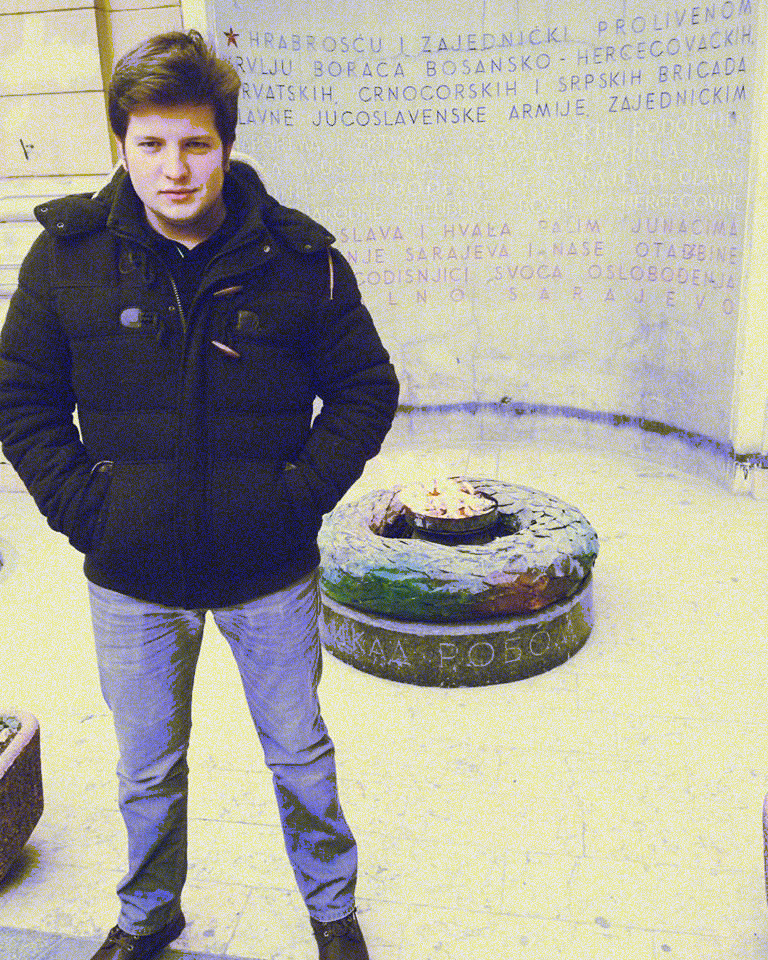
\includegraphics[scale=0.3]{../benchmark_results/pattern/1_components-7_bits.png} \\
1 & 8 &33\% & 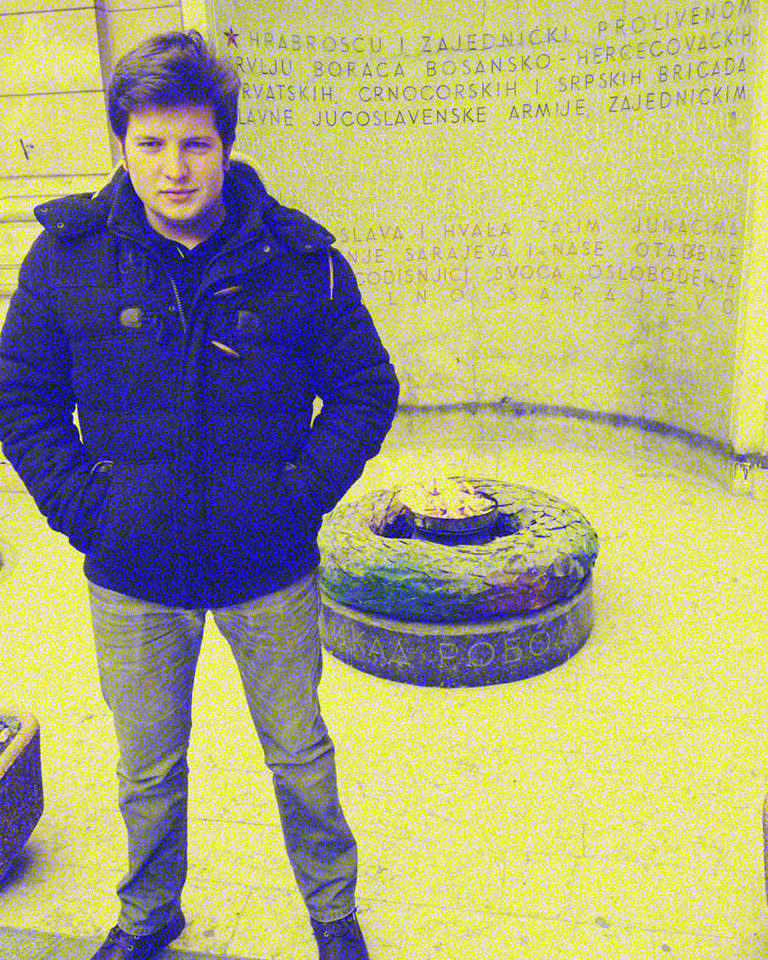
\includegraphics[scale=0.3]{../benchmark_results/pattern/1_components-8_bits.png} \\
2 & 1 &8\% & 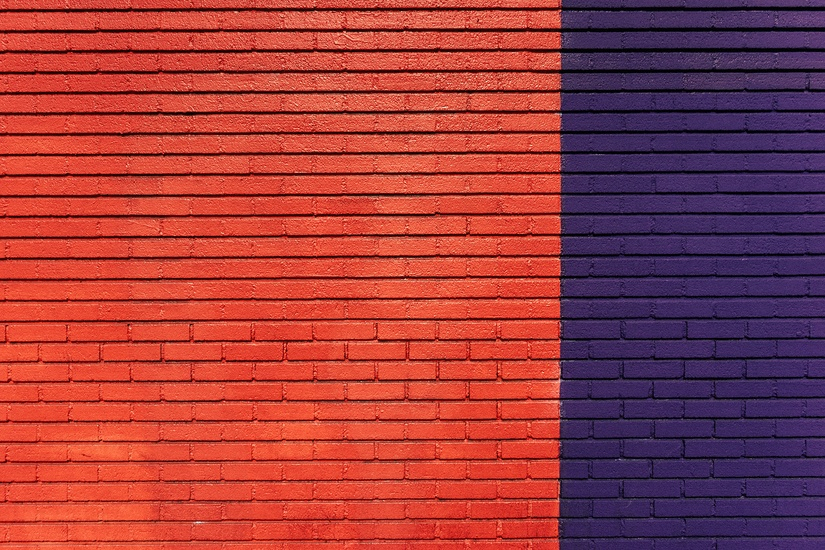
\includegraphics[scale=0.3]{../benchmark_results/pattern/2_components-1_bits.png} \\
2 & 2 &12\% & 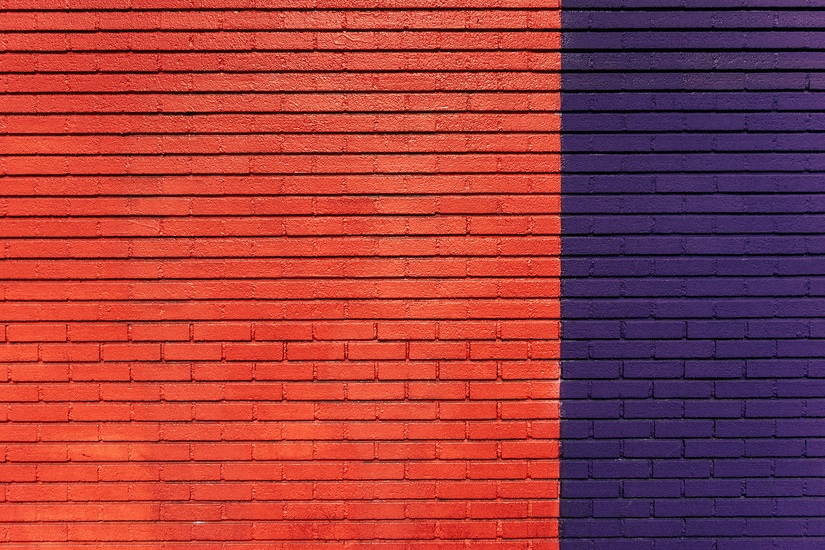
\includegraphics[scale=0.3]{../benchmark_results/pattern/2_components-2_bits.png} \\
2 & 3 &25\% & 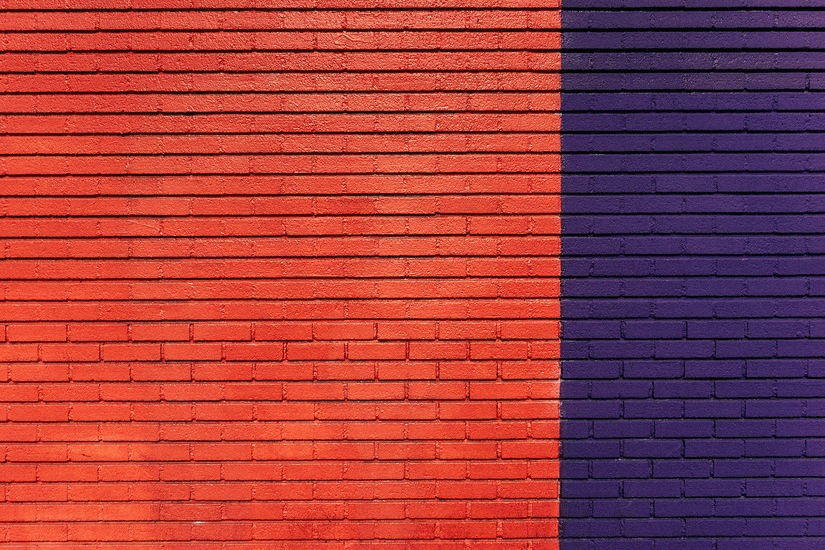
\includegraphics[scale=0.3]{../benchmark_results/pattern/2_components-3_bits.png} \\
2 & 4 &33\% & 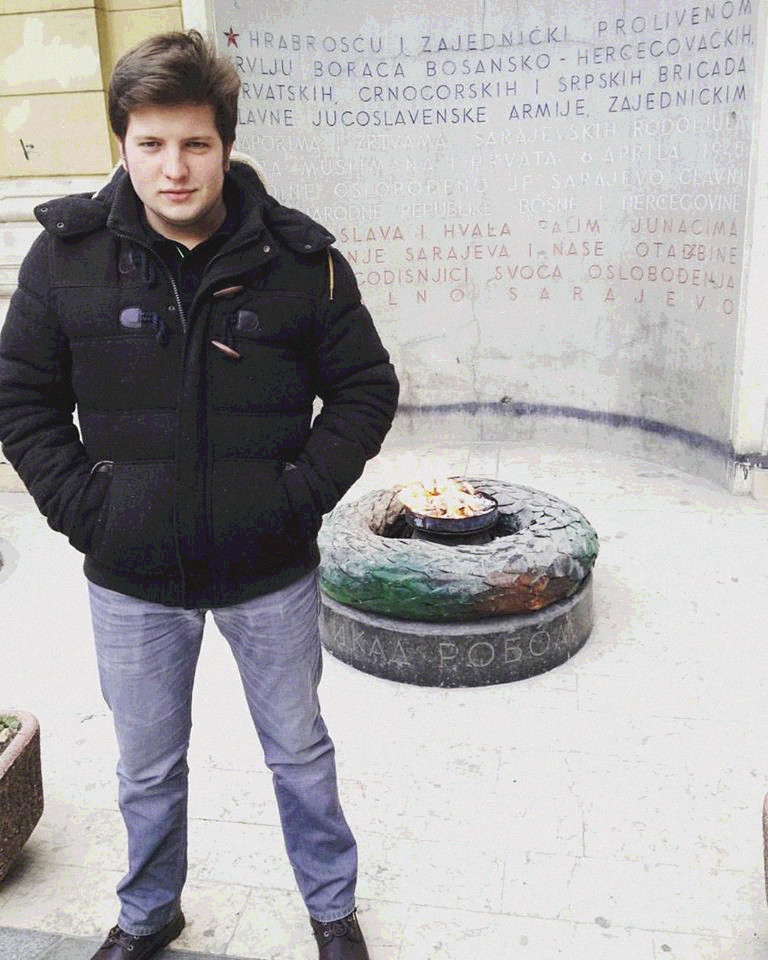
\includegraphics[scale=0.3]{../benchmark_results/pattern/2_components-4_bits.png} \\
2 & 5 &42\% & 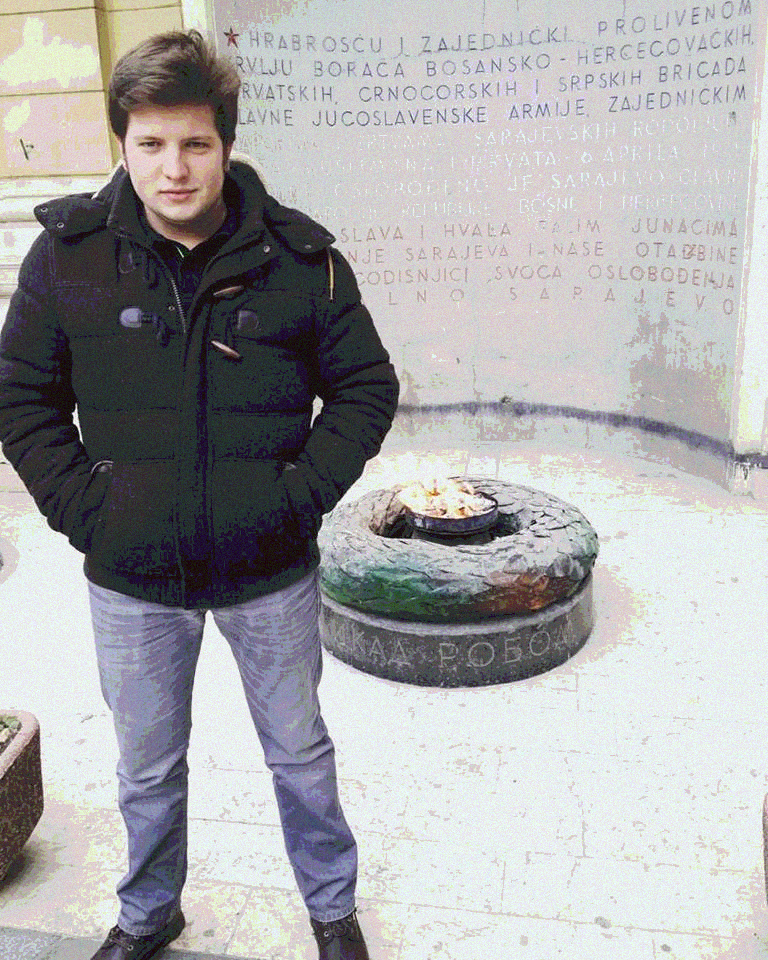
\includegraphics[scale=0.3]{../benchmark_results/pattern/2_components-5_bits.png} \\
2 & 6 &50\% & 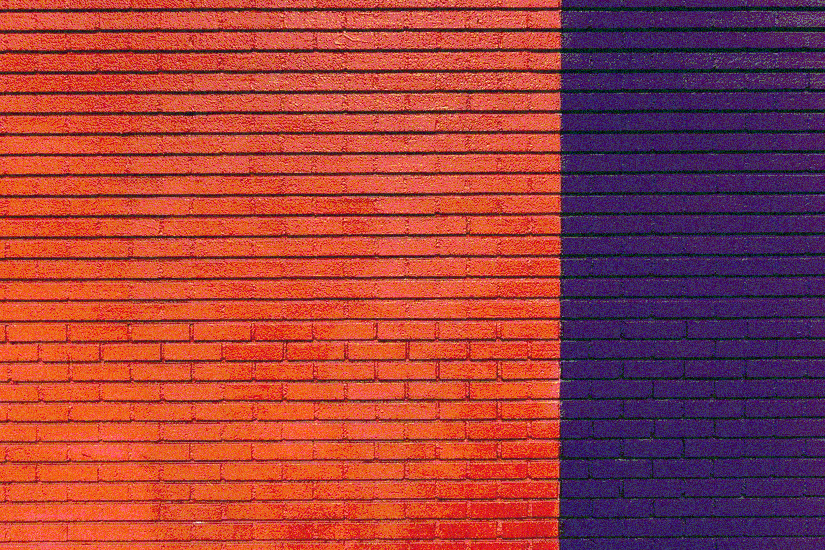
\includegraphics[scale=0.3]{../benchmark_results/pattern/2_components-6_bits.png} \\
2 & 7 &58\% & 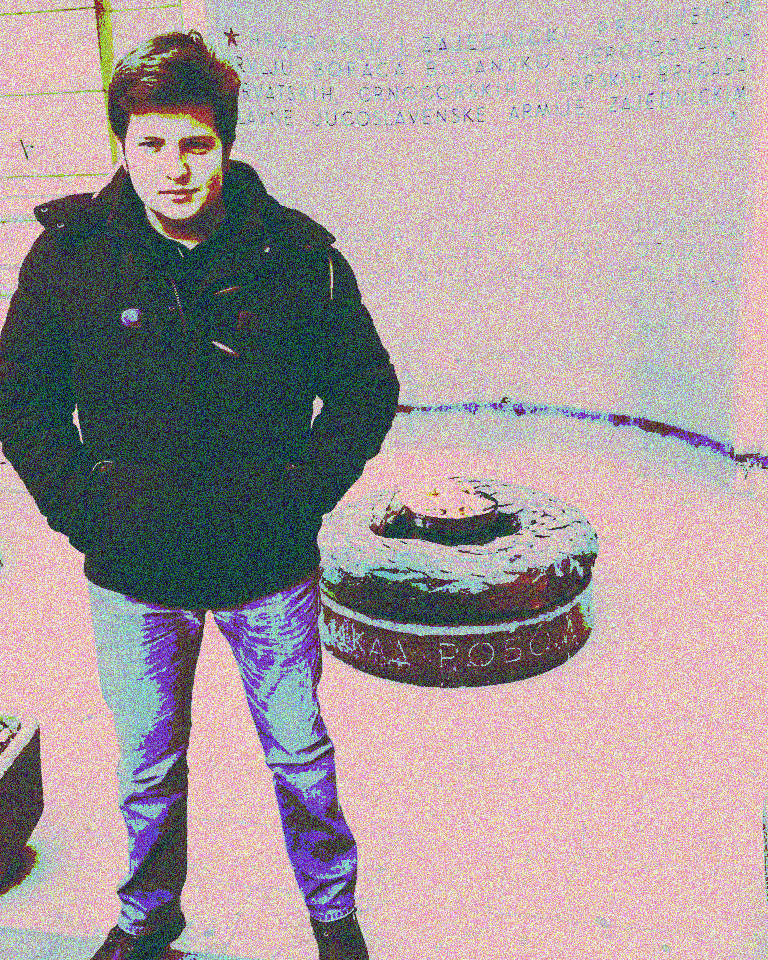
\includegraphics[scale=0.3]{../benchmark_results/pattern/2_components-7_bits.png} \\
2 & 8 &67\% & 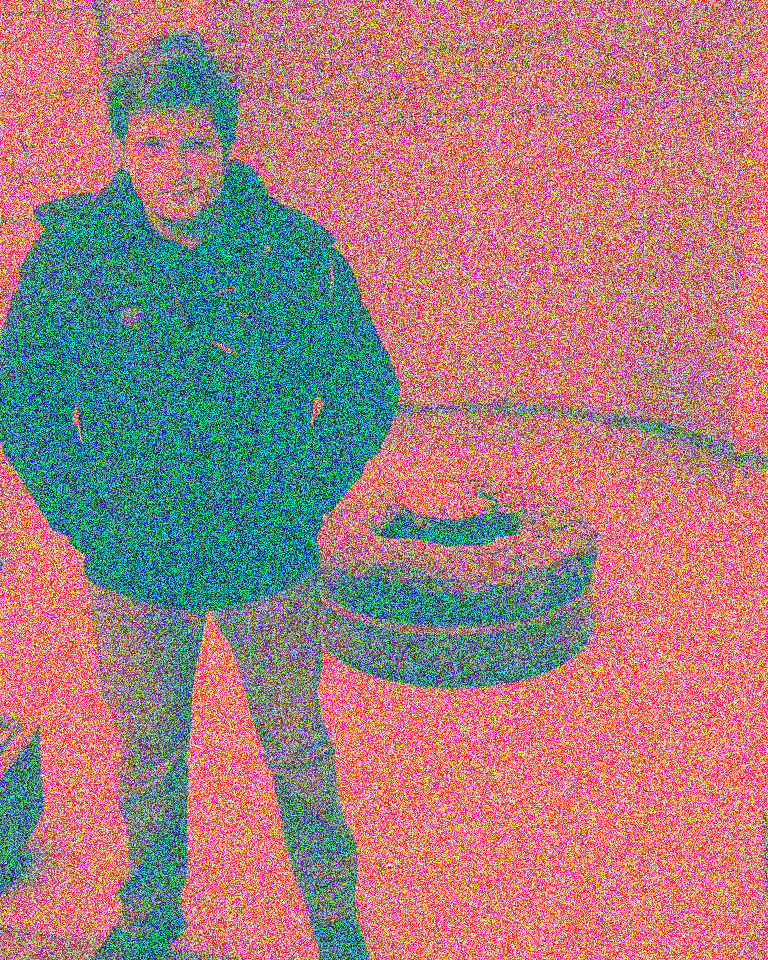
\includegraphics[scale=0.3]{../benchmark_results/pattern/2_components-8_bits.png} \\
3 & 1 &12\% & 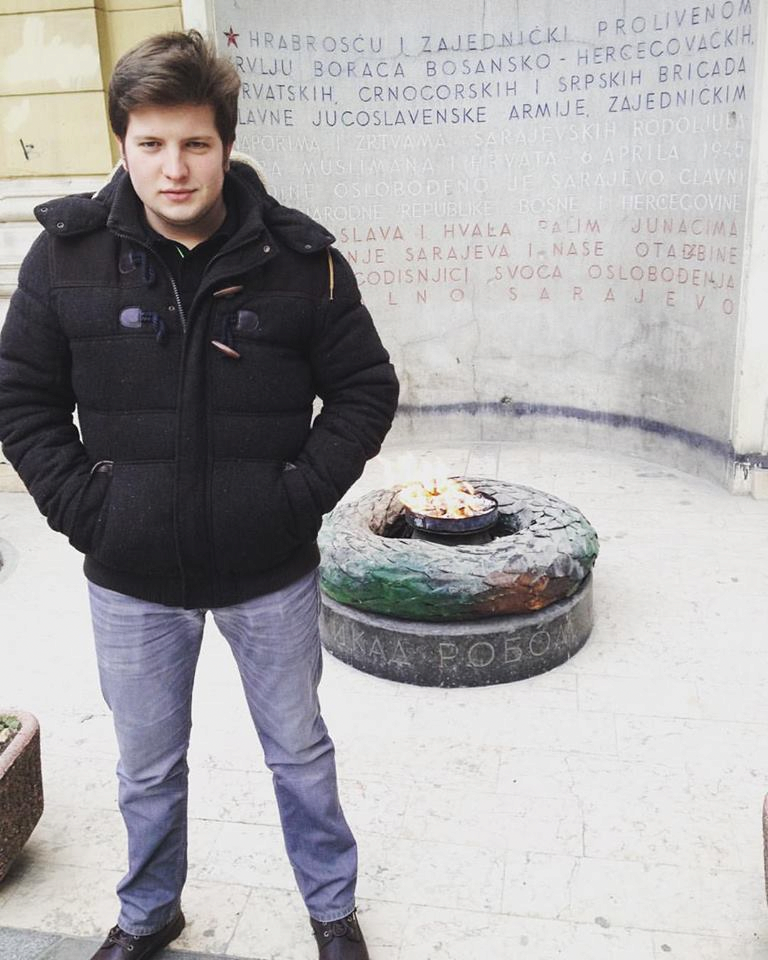
\includegraphics[scale=0.3]{../benchmark_results/pattern/3_components-1_bits.png} \\
3 & 2 &25\% & 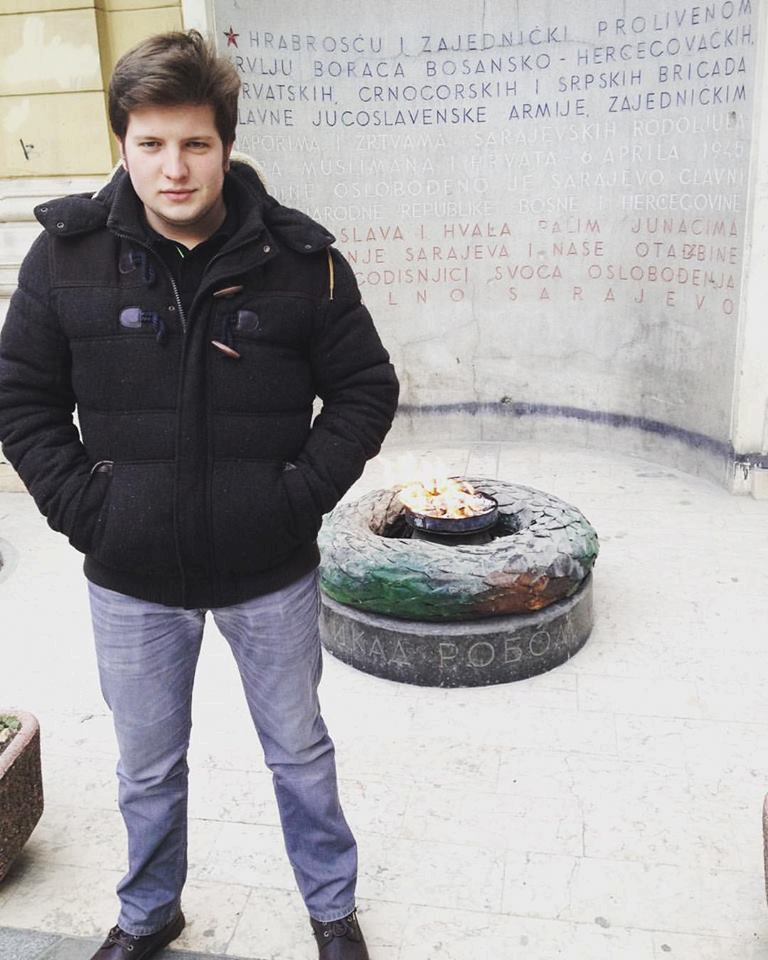
\includegraphics[scale=0.3]{../benchmark_results/pattern/3_components-2_bits.png} \\
3 & 3 &38\% & 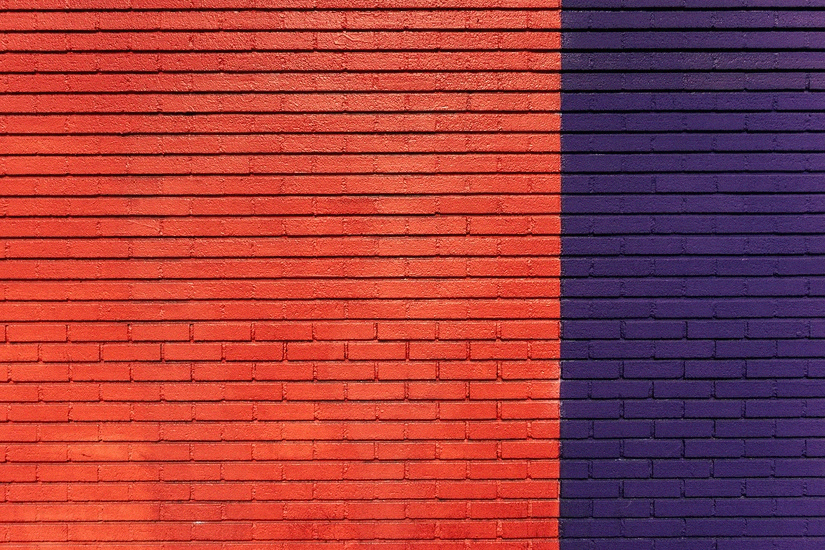
\includegraphics[scale=0.3]{../benchmark_results/pattern/3_components-3_bits.png} \\
3 & 4 &50\% & 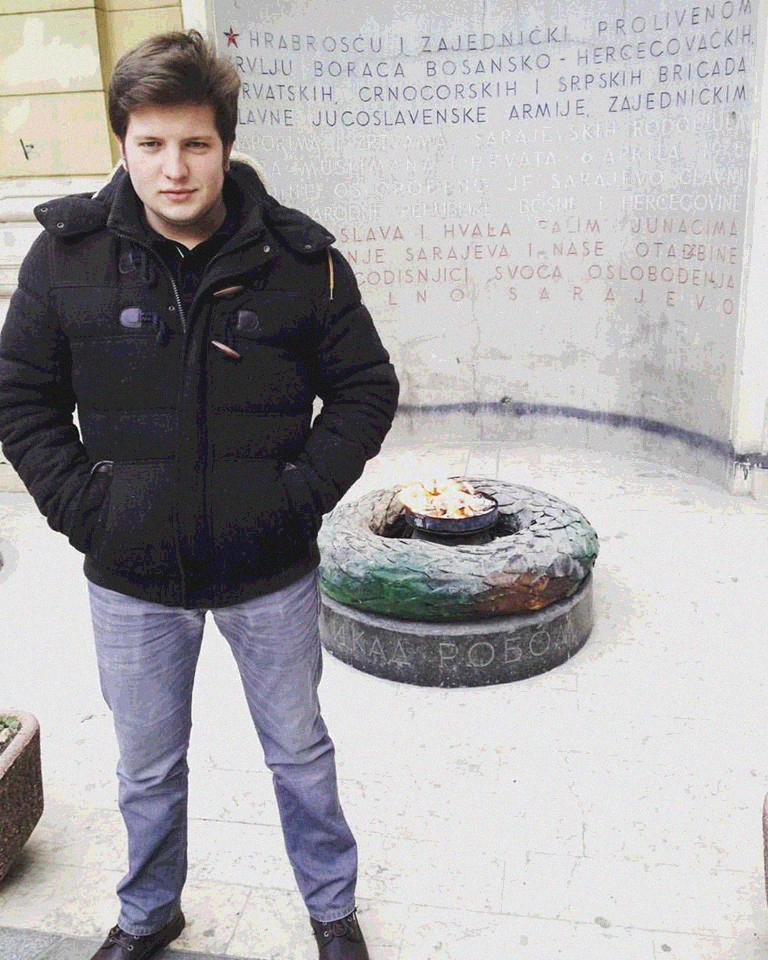
\includegraphics[scale=0.3]{../benchmark_results/pattern/3_components-4_bits.png} \\
3 & 5 &62\% & 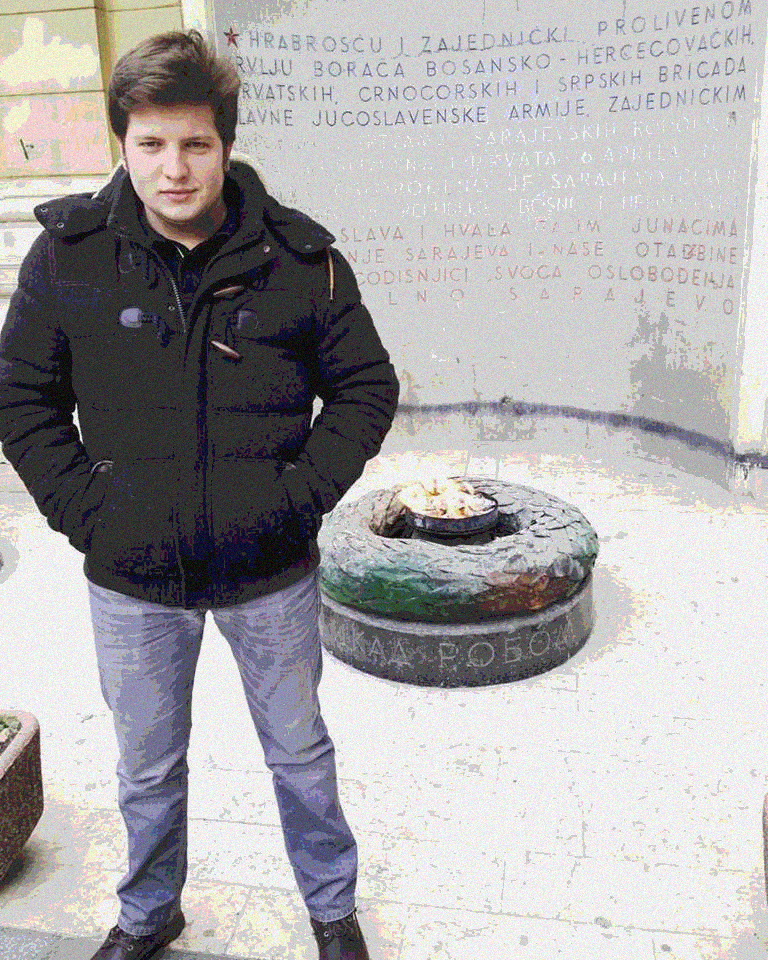
\includegraphics[scale=0.3]{../benchmark_results/pattern/3_components-5_bits.png} \\
3 & 6 &75\% & 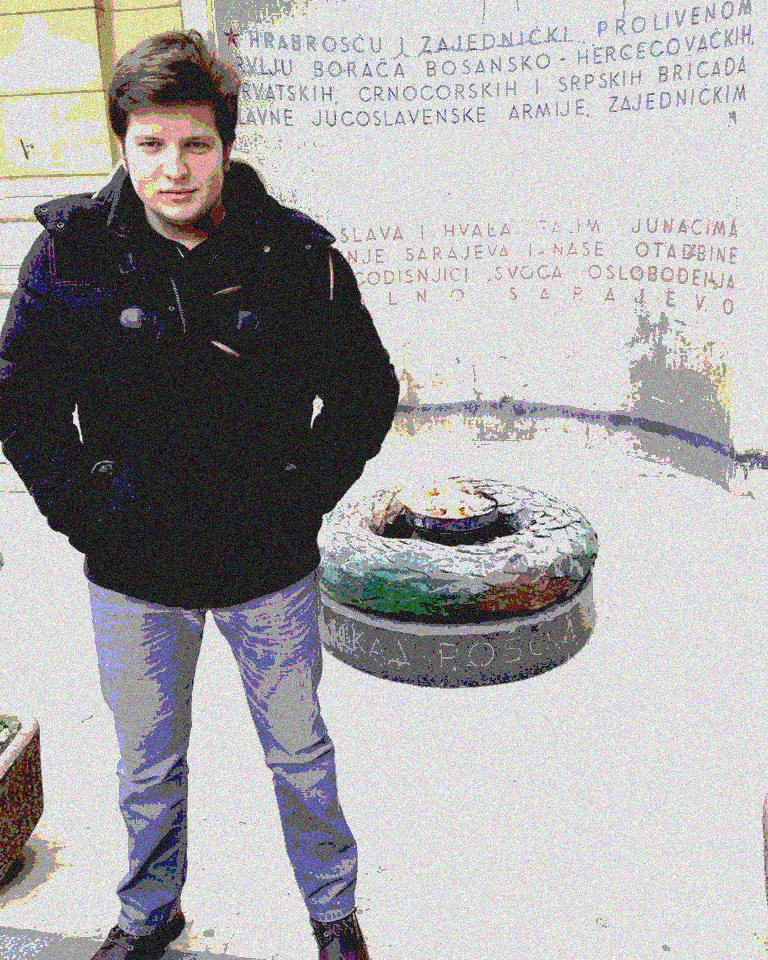
\includegraphics[scale=0.3]{../benchmark_results/pattern/3_components-6_bits.png} \\
3 & 7 &88\% & 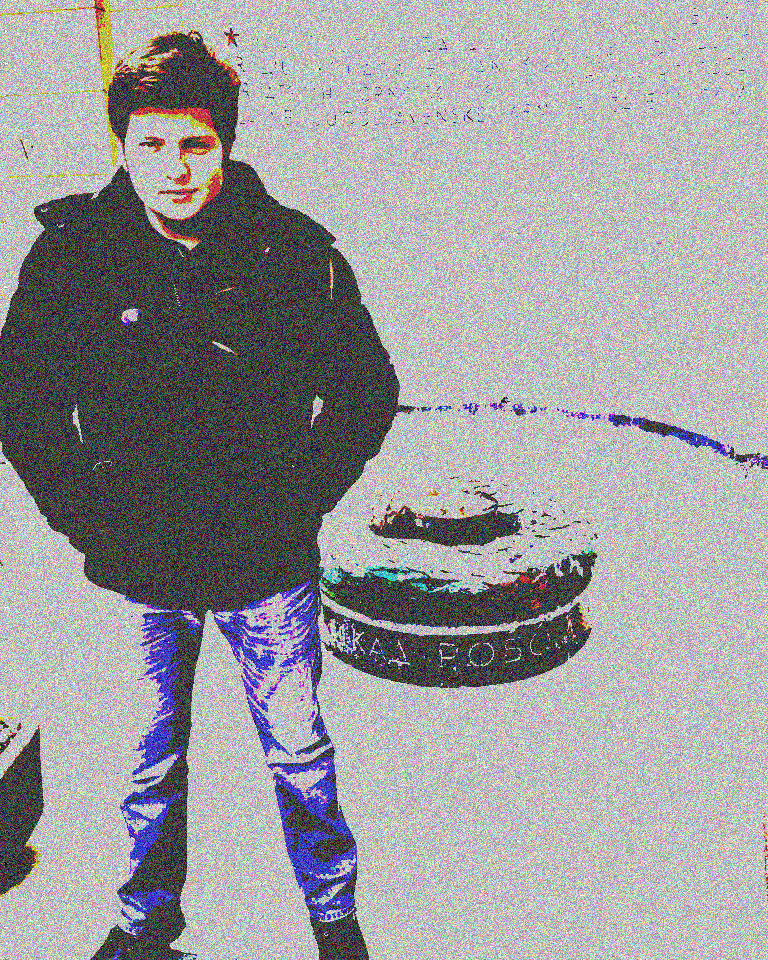
\includegraphics[scale=0.3]{../benchmark_results/pattern/3_components-7_bits.png} \\
3 & 8 &100\% & 
\includegraphics[scale=0.3]{../benchmark_results/pattern/3_components-8_bits.png} \\
\end{longtable}
\end{center}

\section{Analiza rezultata}

\chapter{Opis programske implementacije rješenja}

\chapter{Zaključak}

\bibliography{literatura}
\bibliographystyle{fer}

\end{document}
